\noindent \textbf{ \huge Supplementary Material
%(\#4158)
}

\section{Example of GNN With More Dimensions}

We present an example of GNN with more dimensions, and of a LVP instance, and provide all the details of an instance of computation. We can assume $\setnumbers$ to be the set of signed $4$-bit integers.



\paragraph{GNN $N$.}
Let $N = (\layer_1, \layer_2, \layer_{out})$ be a GNN, such that:
\begin{itemize}
    \item $\layer_1 = (\agg_1, \comb_1)$, $\agg_1 = \sum$, and $\comb_1((x_1, x_2)^T, (\aggvar_1, \aggvar_2)^T) = 
    \begin{pmatrix}
    ReLU(+2x_1 - 1x_2 + 1\aggvar_1 - 1\aggvar_2 - 1) \\
    ReLU(+1x_1 + 2x_2 - 2\aggvar_1 - 1\aggvar_2 + 1)
    \end{pmatrix}$
    \item $\layer_2 = (\agg_2, \comb_2)$,
    $\agg_2 = \sum$, and $\comb_2((x_1, x_2)^T, (\aggvar_1, \aggvar_2)^T) = 
    \begin{pmatrix}
    ReLU(+1x_1 - 1x_2 + 2\aggvar_1 + 2\aggvar_2 - 2) \\
    ReLU(+2x_1 + 0x_2 - 2\aggvar_1 - 1\aggvar_2 + 2) \\
    ReLU(-1x_1 + 1x_2 - 2\aggvar_1 + 1\aggvar_2 - 1)
    \end{pmatrix}$
\end{itemize}
Layer $\layer_1$ has input and output dimensions 2, while layer $\layer_2$ has input dimension 2, and output dimension 3. The output layer $\layer_{out}$ is the identity.


\begin{figure}[h]
    \centering
    	\begin{tikzpicture}
		\draw[fill=white, opacity=0.7,rounded corners = 5mm, draw=none] (-2.5, 1.5) rectangle (0.6, -1.5);
		\node[inner sep=0mm, rounded corners=2mm] (0) at (-2, 0) {\labellednode{v}{1}{1}};
		\node[inner sep=0mm] (1) at (0, 1) {\labellednodeinv{v_1}{0}{1}};
		\node[inner sep=0mm] (2) at (0, -1) {\labellednodeinv{v_2}{1}{0}};
		\draw[->] (0) -- (1);
		\draw[->] (0) edge [bend left=10] (2);
		\draw[->] (1) edge [bend left=10] (2);
		\draw[->] (2) edge [bend left=20] (0);
		
	\end{tikzpicture}
    \caption{The vector-labelled graph $G_e$.}
    \label{fig:graph2}
\end{figure}

\paragraph{Output of $N$ on input $G_e, v$.}
Consider the graph $G_e$ as represented in Figure~\ref{fig:graph2}.

Through the first layer,

$y^0(v) 
= \agg_1(\multiset{x^0(v_1), x^0(v_2)}) 
= \agg_2 (\multiset{(0, 1)^T, (1, 0)^T}) 
= (1,1)^T$

$x^1(v) 
= \comb_1(x^0(v), y^0(v)) 
= \comb_1((1, 1)^T, (1, 1)^T) 
=  \begin{pmatrix}
    ReLU(+2 - 1 + 1 - 1 - 1) \\
    ReLU(+1 + 2 - 2 - 1 + 1)
    \end{pmatrix} 
= (0, 1)^T$


$y^0(v_1) 
= \agg_1(\multiset{}) = (0, 0)^T$

$x^1(v_1) 
= \comb_1(x^0(v_1), \aggvar_0(v_1))
= \comb_1((0,1)^T, (0, 0)^T))
= \begin{pmatrix}
    ReLU(+0 - 1 + 0 - 0 - 1) \\
    ReLU(+0 + 2 - 0 - 0 + 1)
    \end{pmatrix}
= (0, 3)^T$

$y^0(v_2)
= \agg_1(\multiset{(1,1)^T}) = (1, 1)^T$

$x^1(v_2)
= \comb_1(x^0(v_2), \aggvar_0(v_2))
= \comb_1((1,0)^T, (1, 1)^T))
= \begin{pmatrix}
    ReLU(+2 - 0 + 1 - 1 - 1) \\
    ReLU(+1 + 0 - 2 - 1 + 1)
    \end{pmatrix}
= (1, 0)^T$


Through the second layer,

$y^1(v) 
= \agg_2(\multiset{x^1(v_1), x^1(v_2)})
= \agg_2(\multiset{(0,3)^T, (1,0)^T})
= (1,3)^T$

$x^2 (v) 
= \comb_2(x^1(v), y^1(v))
= \comb_2((0,1)^T, (1,3)^T)
= \begin{pmatrix}
    ReLU(+0 - 1 + 2 + 6 - 2) \\
    ReLU(+0 + 0 - 2 - 3 + 2) \\
    ReLU(-0 + 1 - 2 + 3 - 1)
    \end{pmatrix}
= (5,0,1)^T$

% We do not show $x^2(v_1)$ and $x^2(v_2)$.


\paragraph{LVP instance.}
Let $I$ be the LVP instance $(N, L_{in}, L_{out})$, where $N$ is the GNN as defined before, $L_{in} := x_1 + x_2 \geq x_1 + x_2$, and $L_{out} := y_1 - y_2 - y_3 \geq 0$. (The linear inequality $L_{in}$ is tautological.)

$(G_e, v) = (1,1)^T$ satisfies $L_{in}$ and $N(G_e,v) = (5,0,1)^T$ satisfies $L_{out}$.

But $I$ is not valid.
To see that, consider the graph $G$ that has only one vertex $v$, labelled $\ell(v) = \begin{pmatrix}
        0\\0
\end{pmatrix}$.

Through the first layer,

$y^0(v) 
= (0,0)^T$

$x^1(v)
=  \begin{pmatrix}
    ReLU(- 1) \\
    ReLU(+ 1)
    \end{pmatrix} 
= (0, 1)^T$

Through the second layer,

$y^1(v) 
= (0,0)^T$

$x^2 (v) 
= \begin{pmatrix}
    ReLU(- 1 - 2) \\
    ReLU(+ 0 + 2) \\
    ReLU(+ 1 - 1)
    \end{pmatrix}
= (0,2,0)^T$

$(G, v) = (0,0)^T$ satisfies $L_{in}$ but $N(G,v) = (0,2,0)^T$ does not satisfy $L_{out}$.

















\section{Omitted Proofs}






\subsection{Proof of \Cref{th:satlogPSPACE} (Arity in Binary or Unbounded)}
\label{sec:proofs-arity-binary-or-unbounded}

In this subsection, we prove that \Cref{th:satlogPSPACE} holds when the arity is written in binary or is unbounded ($\arity = +\infty$). The unbounded case still means that the branching is finite at each node but unbounded. We prove PSPACE membership by adapting the tableau rules given in Figure~\ref{figure:tableaurules}. The new tableau rules will work both for the cases when the arity is written in binary and the case when it is unbounded ($\arity = +\infty$).

 

 \paragraph{Rule for guessing the arity.} First, we modify the rule $(arity)$ as follows:
	
	
	\begin{prooftree}
		\AxiomC{$(w~\phi)$ and no term $(w~arity=..)$}
		\rulelabel{arity}
		\UnaryInfC{$(w~arity=\delta')$ for some $\delta'\leq \delta$ with $\delta' \leq 2^n |\phi|$}
	\end{prooftree}
%	
	where this time $\delta'$ is written in binary. The rule $(arity)$ works when $\delta$ is an integer or $+\infty$.
% \todo{Can we actually handle infinite branching? Or need $\delta' < \delta$, when $\delta = \inf$? Logic has finite-braching/model property, right?} 
 %yes, it is FINITE branching but unbounded one.
In the above rule, we guess the arity of a node $w$ to be bounded by $\delta$ like in the rule in~\Cref{figure:tableaurules}. But, we additionally suppose that $\delta'$ is an integer between $0$ and $2^n |\phi|$ written with $O(n \log |\phi|)$ bits. Why is the bound $2^n |\phi|$ sufficient? The idea is that having $\delta'$ greater than $2^n |\phi|$ is useless because $2^n |\phi|$ is a bound for having all the combinations for $\expression_1 = k_1, \dots, \expression_m = k_m$ for $\agg(\expression_1), \dots, \agg(\expression_m)$ appearing in $w$ (we thus have $m \leq |\phi|)$.

	
% \todo{arity unbounded starts here? }
%François: No it is the same proof for delta an integer or delta = +infty



\paragraph{Rules for aggregation. }
Whereas there is a single rule $(\agg)$ in Figure~\ref{figure:tableaurules} for handling the aggregation, we will introduce three rules.

	First, we add the following rule that initializes the computation for $\agg(\expression) = k$:
	
	\begin{prooftree}
		\AxiomC{$(w~\agg(\expression) = k)$}
		\rulelabel{\agg_{init}}
		\UnaryInfC{
			$(w~~0~~\agg(\expression) = k~~0)$
		}
	\end{prooftree}
	
	The term $(w~~i~~\agg(\expression) = k~~A)$ indicates that we have already performed the computation for the successors $w1, \dots, wi$ and the cumulative sum so far is $A$. With the rule $(\agg_{init})$, it means that we did not consider any successors so far and the cumulative sum so far is zero.
	
	%The following rule means that we successfully stop the process if we reached the value $k$ with the given arity $\delta'$:
 %\todo{I don't think this is needed}
 
	%\begin{prooftree}
	%	\AxiomC{$(w~~arity = \delta')~~ (w~~\delta'~~agg(\expression) = k~~k)$}
	%	\rulelabel{agg_{stop}}
	%	\UnaryInfC{
	%	}
	%\end{prooftree}

%François: I agree, we do not need it since the rule does not produce anything.. so.... just do nothing :) Thank you!

The next rule $(agg_{rec})$ is the \emph{recursive} rule and treats the $i$-th successor as follows. It guesses the value $k'$ for feature $\expression$ for the successor $w(i+1)$. It updates the cumulative result so far to $A+k'$.
	
	\begin{prooftree}\small
		\AxiomC{\begin{minipage}{0.8\linewidth}$(w~~i~~\agg(\expression) = k ~~A)~~ (w~~arity=\delta')$ with $i<\delta'$
  \end{minipage}}
		\rulelabel{agg_{rec}}
		\UnaryInfC{\begin{minipage}{0.8\linewidth}
			$(w(i+1)~~\expression {=} k')~~(w~~i{+}1~~\agg(\expression) = k~~A+k')$ for some $k'$
\end{minipage}		
  }
	\end{prooftree}

    
 The last rule $(agg_{fail})$ says that the tableau method fails if the cumulative value $A$ obtained when all the successors $w1, \dots, w\delta'$ have been considered is different from the expected $k$:
	
	
	\begin{prooftree}\small
		\AxiomC{\begin{minipage}{0.8\linewidth}
  $(w~~arity = \delta')~~ (w~~\delta'~~\agg(\expression) = k~~A)$ with $A \neq k$
  \end{minipage}
  }
		\rulelabel{agg_{fail}}
		\UnaryInfC{fail
		}
	\end{prooftree}
	
	
	
	

	
	The procedure can still be executed in PSPACE by exploring the successors in a depth-first-search manner. We treat each successor one after another. After treating $wi$ completely, we free the memory for the whole computation for successor $wi$.














\subsection{Proof of \Cref{lemma:GMLonegrapharitytwo}}

Before proving \Cref{lemma:GMLonegrapharitytwo} we focus on modal logic over graphs of arity at most $2$.


\subsubsection{Modal logic over graphs of arity at most $2$}

Similarly to standard modal logic, the satisfiability problem of modal logic over the class of graphs of arity at most $2$, that we denote by $\Ktwoa$, is also PSPACE-hard. Its proof is similar to the one for standard modal logic in \citet{DBLP:books/cu/BlackburnRV01}.


\begin{lemma}
	\label{lemma:K2a}
    The satisfiability problem of $\Ktwoa$ is PSPACE-hard.
\end{lemma}


\begin{proof}
	By poly-time reduction from TQBF. As said, the proof follows the proof of PSPACE-hardness of modal logic K \cite{DBLP:books/cu/BlackburnRV01}. We give the main argument in order to be self-contained.
	
	Let us take a quantified binary formula $\exists p_1 \forall p_2 \dots \exists p_{2n-1} \forall p_{2n} \chi$ where $\chi$ is propositional.
	The game behind TQBF can be represented by the binary tree in which $p_i$ is chosen at the $i$-th level.
	
	
	
	Modal logic, even restricted to models of arity bounded by $2$, can express that the Kripke model contains this binary tree. The following formula explains how the $i$-th level should look like:
%
 $$\lbox ^i \left( \ldiamond p_i \land \ldiamond \lnot p_i \land \lbigand_{j<i} (p_j \lequiv \lbox p_j) \right)$$
	
	
	Let $TREE$ be the conjunction of the above formulas for $i=1..2n$ that forces the Kripke model to contain the binary tree up to level $2n$ (see Figure~\ref{fig:binarytreeforTQBF}). On the input $\exists p_1 \forall p_2 \dots \exists p_{2n-1} \forall p_{2n} \chi$, the reduction computes in polynomial time the modal formula $TREE \land \ldiamond \lbox \dots \ldiamond \lbox \chi$. The former is true iff the latter is satisfiable.
	
	
	\begin{figure*}[ht]
		\begin{center}
			\scalebox{0.8}{
				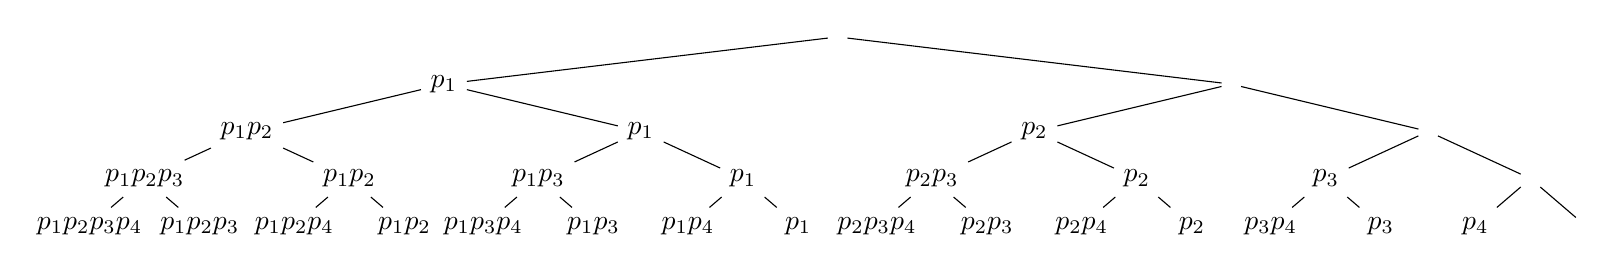
\begin{tikzpicture}[yscale=0.4, xscale=1, level distance=15mm,
					level 4/.style={sibling distance=14mm},
					level 3/.style={sibling distance=26mm},
					level 2/.style={sibling distance=50mm},
					level 1/.style={sibling distance=100mm},
					]
					\node {}
					child { node {$p_1$} 
						child { node {$p_1p_2$}
							child {node {$p_1p_2p_3$}
								child {node {$p_1p_2p_3p_4$}}
								child {node {$p_1p_2p_3$}}
							}
							child {node {$p_1p_2$}
								child {node {$p_1p_2p_4$}}
								child {node {$p_1p_2$}}
							}
						}
						child { node {$p_1$}
							child {node {$p_1p_3$}
								child {node {$p_1p_3p_4$}}
								child {node {$p_1p_3$}}
							}
							child {node {$p_1$}
								child {node {$p_1p_4$}}
								child {node {$p_1$}}
							}
						}
					}
					child { node {} 
						child { node {$p_2$}
							child {node {$p_2p_3$}
								child {node {$p_2p_3p_4$}}
								child {node {$p_2p_3$}}
							}
							child {node {$p_2$}
								child {node {$p_2p_4$}}
								child {node {$p_2$}}
							}
						}
						child { node {}
							child {node {$p_3$}
								child {node {$p_3p_4$}}
								child {node {$p_3$}}
							}
							child {node {}
								child {node {$p_4$}}
								child {node {}}
							}
						}
					};
			\end{tikzpicture}}
		\end{center}
		
		\caption{Binary tree for a TQBF game for $n=2$ (i.e., variables $p_1, p_2, p_3, p_4$. The value of $p_1$ is chosen at the root. The value of $p_2$ is chosen at depth 1, etc.}
		\label{fig:binarytreeforTQBF}
	\end{figure*}
	
\end{proof}


\subsubsection{Proof of \Cref{lemma:GMLonegrapharitytwo}}


%\begin{lemma}
%The satisfiability of $\fragmentGMLmodallogic$ on graphs of arity at most $2$ is PSPACE-hard.
%\label{lemma:GMLonegrapharitytwo}
%\end{lemma}

\begin{proof}
\fbox{$\fragmentGMLmodallogic$ on graphs of arity at most 2}
We reduce the satisfiability problem of $\Ktwoa$ (which is PSPACE-hard, see \Cref{lemma:K2a}) to the satisfiability problem of $\fragmentGMLmodallogic$ on graphs of arity at most 2.
We translate modal logic into GML as follows: $tr(p) = p$ and $tr(\lbox \phi) = \lnot \gmlbox 1 \lnot tr(\phi)$. In other words, $\lbox \phi$ is translated as `it is false that there is no successor with $tr(\phi)$ false'.


\fbox{$\fragmentGML$}
We reduce the satisfiability problem of $\Ktwoa$ (which is PSPACE-hard, see \Cref{lemma:K2a}) to the satisfiability problem of $\fragmentGML$.
We can prove that  we can express that the arity is bounded by $2$ in $\fragmentGML$.

	We then define $\tau(\phi) = tr(\phi) \land \lbigand_{i=0}^d (\lnot \gmlbox 1\lnot )^i \lnot \gmlbox 3 \top$
    where $d$ is the modal depth of $\phi$, and where $tr$ is the translation given in the proof of \Cref{lemma:GMLonegrapharitytwo}. 
    
    The subformula $\lnot \gmlbox 3 \top$ says that it is false that there are at least~3 successors.
	The subformula $\lbigand_{i=0}^d (\lnot \gmlbox 1\lnot )^i \lnot \gmlbox 3 \top$ says that the vertices should have at most 2 successors, up to the modal depth of $\phi$.
	
	Now it can be proven by induction on $\phi$ that 
	$\phi$ is $\Ktwoa$-satisfiable iff $tr(\phi)$ is $\fragmentGML$-satisfiable.
\end{proof}








\subsection{Proof of \Cref{corollary-satthelogicPSPACEc}}


\begin{proof}
      PSPACE membership is stated in Theorem~\ref{th:satlogPSPACE}. Hardness is proven by the poly-time reduction (see Theorem~\ref{th:reduction}) from LVP (which is PSPACE-hard in this context, see \Cref{theorem:LVPPSPACEcomplete}) to the satisfiability problem of~\thelogic{}. 
\end{proof}

\begin{corollary}
The satisfiability problem of \thelogic{} is PSPACE-complete, and already PSPACE-hard in the restrictive cases and if the activation function is ReLU.
\end{corollary}

\begin{proof}
    It suffices to observe that truncated ReLU can be simulated as follows:
    %
    $truncatedReLU(x) := RelU(ReLU(x) - ReLU(x-1))$.
%
    So we can reduce the satisfiability problem of \thelogic{} with truncated ReLU to the satisfiability problem of \thelogic{} with ReLU. To do that, we replace each occurrence of $\activationfunction(E)$ (where $\activationfunction$ was previously interpreted as truncated ReLU) by $\activationfunction(\activationfunction(E) - \activationfunction(E-1))$ (where now $\activationfunction$ is interpreted as ReLU). This operation does not blow up the size of the formula since formulas are represented by DAGs. 
\end{proof}
















\section{Discussion on Other Aggregation Functions}
\label{appendix-section-aggregation}

In this section, we show how our methodology can be easily applied for other aggregation functions, like those, for instance, compared in \citet{RosenbluthTG23}. The idea is to replace the $\agg$ operator.
\paragraph{Weighted sum in aggregation functions}

%https://cs.mcgill.ca/~wlh/comp766/files/chapter4_draft_mar29.pdf
%Veliˇckovi´c et al. [2017]’s Graph Attention Network (GAT), 
In variants of GNN, the summation in the aggregation function is weighted (e.g. \cite{DBLP:conf/iclr/VelickovicCCRLB18}). Assuming that the weights are fixed for each edge, we can replace operator $\agg$ with $\agg_{\textsf w_1\dots \textsf w_\delta}$ where  $\textsf w_1\dots \textsf w_\delta$ are weights. The rule will then have the form:
\begin{prooftree}
\AxiomC{$(w~\agg_{\textsf w_1\dots \textsf w_\delta}(\expression) = k)$}
\AxiomC{$(w~arity=\delta')$}
\rulelabel{\agg_{\vec{\textsf w}}}
\BinaryInfC{
\begin{minipage}{0.4\textwidth}
$(w1~\expression = k_{1}), \dotsc, (w \arity'~\expression = k_{{\arity'}})$ for some $(k_u)_{u=1..\arity'}$, with $\textsf w_1 k_{1} +_{\setnumbers_n} 
 \dotsb +_{\setnumbers_n} \textsf w_{\arity'} k_{\arity'} = k$
\end{minipage}
}
\end{prooftree}

\paragraph{Max-GNNs}

In Max-GNNs (\cite{DBLP:conf/kr/CucalaG24}), the aggregation function is the maximum. Our framework can be adapted by replacing the operator $\agg$ with $\max$. We then use the following rule:
\begin{prooftree}
\AxiomC{$(w~\max(\expression) = k)$}
\AxiomC{$(w~arity=\delta')$}
\rulelabel{\max}
\BinaryInfC{
\begin{minipage}{0.4\textwidth}
$(w1~\expression = k_{1}), \dotsc, (w \arity'~\expression = k_{{\arity'}})$ for some $(k_u)_{u=1..\arity'}$, with $\max(k_{1},
 \dotsb, k_{\arity'}) = k$
\end{minipage}
}
\end{prooftree}

\paragraph{Mean-GNNs}

In Mean-GNNs (\cite{RosenbluthTG23}), the aggregation function is the average. We can adapt our framework replacing the operator $\agg$ with $mean$.
It can scale better than sum aggregation across nodes with varying arity. 
The behavior of this aggregation function is captured by the following rule:
\begin{prooftree}
\AxiomC{$(w~mean(\expression) = k)$}
\AxiomC{$(w~arity=\delta')$}
\rulelabel{mean}
\BinaryInfC{
\begin{minipage}{0.4\textwidth}
$(w1~\expression = k_{1}), \dotsc, (w \arity'~\expression = k_{{\arity'}})$ for some $(k_u)_{u=1..\arity'}$, with $(k_{1} +_{\setnumbers_n} 
 \dotsb +_{\setnumbers_n} k_{\arity'}) /_{\setnumbers_n} \arity' = k$
\end{minipage}
}
\end{prooftree}

\medskip
In every case, this yields a PSPACE decision procedures for satisfiability and validity checking. In the case of weighted sum, this complexity is tight.




\section{Implementation}
\label{appendix-section-implementation}

We provide a Python implementation of our tableau method where the set of numbers is of the form $\setnumbers_a := \set{-a, -a+1, \dots, 0, 1, \dots, a-1, a}$ where overflows are handled as follows: $x+_\setnumbers y = \max(-a, \min(a, x+y))$.
%\todo{a little lie? We discard something like $a+1$ in the implementation, while here we claim that $a+1 = ... = a + a = a$.}
We also assume $\arity = 2$.

The implementation relies on pattern matching available in Python 3.10 for implementing the tableau rules.

Formulas are written by means of Python tuples. Here is an example of an input formula \texttt{phi}:

\begin{scriptsize}
\begin{verbatim}
phiIn = (("agg", "x1"), ">=", 1)
phiN = (
    ((("ReLU", ("*", 2, "x1")), "-", "y1"), "=", 0),
    "and",
    ((("*", 2, ("agg", "x1")), "-", "y2"), "=", 0)
)
phiOut = ("y1", ">=", 1)
phi = ((phiIn, "and", phiN), "and", ("not", phiOut))
\end{verbatim}
\end{scriptsize}


The program starts with a single set of terms:

\begin{scriptsize}
\begin{verbatim}
{(1, phi)}
\end{verbatim}
\end{scriptsize}

Then the program applies the rules:

\begin{scriptsize}
\begin{verbatim}
initialization:  {(1, (((('agg', 'x1'), '>=', 1), 
'and', (((('ReLU', ('*', 2, 'x1')), '-', 'y1'), '=', 0),
'and', ((('*', 2, ('agg', 'x1')), '-', 'y2'), '=', 0))),
'and', ('not', ('y1', '>=', 1))))}
apply ruleAnd : {(1, ((('agg', 'x1'), '>=', 1), 'and', 
(((('ReLU', ('*', 2, 'x1')), '-', 'y1'), '=', 0), 'and',
((('*', 2, ('agg', 'x1')), '-', 'y2'), '=', 0)))),
(1, ('not', ('y1', '>=', 1)))}
apply ruleAnd : {(1, (('agg', 'x1'), '>=', 1)),
(1, (((('ReLU', ('*', 2, 'x1')), '-', 'y1'), '=', 0), 
'and', ((('*', 2, ('agg', 'x1')), '-', 'y2'), '=', 0))),
(1, ('not', ('y1', '>=', 1)))}
apply ruleAnd : {(1, (('agg', 'x1'), '>=', 1)),
(1, ((('ReLU', ('*', 2, 'x1')), '-', 'y1'), '=', 0)),
(1, ((('*', 2, ('agg', 'x1')), '-', 'y2'), '=', 0)),
(1, ('not', ('y1', '>=', 1)))}
apply ruleNot : 
{(1, ((('*', 2, ('agg', 'x1')), '-', 'y2'), '=', 0)), 
(1, (('*', -1, 'y1'), '>=', -1)),
(1, ((('ReLU', ('*', 2, 'x1')), '-', 'y1'), '=', 0)),
(1, (('agg', 'x1'), '>=', 1))}
new branch:
{(1, ((('*', 2, ('agg', 'x1')), '-', 'y2'), '=', 0)),
(1, (('*', -1, 'y1'), '=', -1)), 
(1, ((('ReLU', ('*', 2, 'x1')), '-', 'y1'), '=', 0)), 
(1, (('agg', 'x1'), '>=', 1))}
new branch:  
{(1, ((('*', 2, ('agg', 'x1')), '-', 'y2'), '=', 0)),
(1, ((('ReLU', ('*', 2, 'x1')), '-', 'y1'), '=', 0)),
(1, (('*', -1, 'y1'), '=', 0)), (1, (('agg', 'x1'), '>=', 1))}
...
\end{verbatim}
\end{scriptsize}


On that example, the program stops by giving a set of terms:

\begin{scriptsize}
\begin{verbatim}
no more rules applicable
example of final tableau: 
{(12, ('x1', '=', 4)),
(11, ('x1', '=', -3)),
(1, ('x1', '=', -2)),
(1, ('y1', '=', 0)),
(1, ('y2', '=', 2))}
\end{verbatim}
\end{scriptsize}
from which we get a pointed labelled graph
\begin{center}
    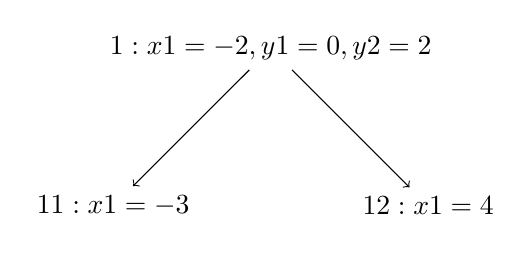
\begin{tikzpicture}
        \node (1) {$1: x1 = -2, y1 = 0, y2 = 2$};
        \node (11) at (-2, -2) {$11: x1 = -3$};
        \node (12) at (2, -2) {$12: x1 = 4$};
        \draw (1) edge[->] (11);
        \draw (1) edge[->] (12);
    \end{tikzpicture}
\end{center}
that satisfies the input formula.

% In \Cref{fig:runtime}, we report 
We report a basic performance evaluation on a MacBook Apple M3 Pro with 36GB memory. It displays the time for running the tableau method starting with the formula \texttt{phi}, for varying values of $a$, hence using numbers in $\setnumbers_a$.
%\begin{figure}

\medskip

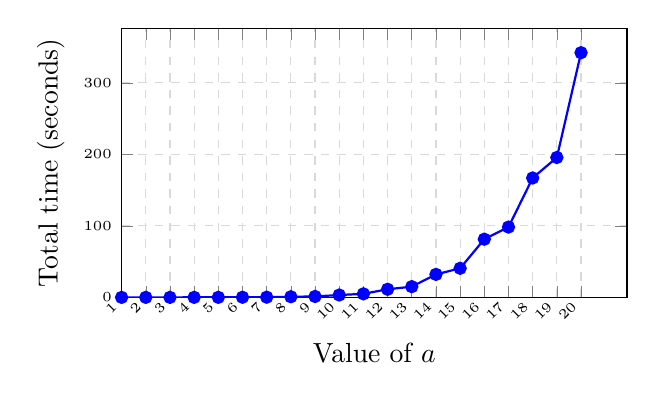
\begin{tikzpicture}[]
    \begin{axis}[
        xlabel={Value of $a$},
        ylabel={Total time (seconds)},
        grid=both,
        grid style={dashed, gray!30},
        ymin=0,
        xmin=1,
        xtick={1,2,3,4,5,6,7,8,9,10,11,12,13,14,15,16,17,18,19,20},
        xticklabel style={rotate=45, anchor=east},
        ticklabel style={font=\tiny},
        width=8cm,
        height=5cm,
        title={}
    ]
        \addplot[
            thick,
            color=blue,
            mark=*,
            mark options={solid, fill=blue}
        ]
        coordinates {
            (1, 0.040)
            (2, 0.042)
            (3, 0.048)
            (4, 0.064)
            (5, 0.088)
            (6, 0.201)
            (7, 0.299)
            (8, 0.900)
            (9, 1.290)
            (10, 3.345)
            (11, 4.978)
            (12, 11.353)
            (13, 15.012)
            (14, 32.158)
            (15, 40.698)
            (16, 81.39)
            (17, 98.33)
            (18, 167.00)
            (19, 195.67)
            (20, 342.18)
        };
    \end{axis}
\end{tikzpicture}

%     \caption{Running time for running the tableau method with the formula \texttt{phi} for varying values of $a$, hence using numbers in $\setnumbers_a$.\label{fig:runtime}}
% \end{figure}